\documentclass[a4paper,11pt]{article}%

\usepackage{fullpage}%
\usepackage[T1]{fontenc}%
\usepackage[utf8]{inputenc}%
\usepackage[main=francais,english]{babel}% % Adjust the main language

\usepackage{graphicx}%
\usepackage{url}%
\usepackage{abstract}%

\usepackage{amsmath}%
\usepackage{subfig}%

\usepackage{newpxtext, newpxmath}

\usepackage{listings}%
\usepackage{xcolor}%
% \definecolor{blue}{0,0,0.8}
% \definecolor{green}{0,0.7,0}
% \definecolor{blue}{0.58,0,0.82}

\lstset{%
  basicstyle=\sffamily,%
  columns=fullflexible,%
  language=R,%       % Adjust according to your current language
  frame=lb,%
  frameround=fftf,%
  literate=
  {á}{{\'a}}1 {é}{{\'e}}1 {í}{{\'i}}1 {ó}{{\'o}}1 {ú}{{\'u}}1
  {Á}{{\'A}}1 {É}{{\'E}}1 {Í}{{\'I}}1 {Ó}{{\'O}}1 {Ú}{{\'U}}1
  {à}{{\`a}}1 {è}{{\`e}}1 {ì}{{\`i}}1 {ò}{{\`o}}1 {ù}{{\`u}}1
  {À}{{\`A}}1 {È}{{\'E}}1 {Ì}{{\`I}}1 {Ò}{{\`O}}1 {Ù}{{\`U}}1
  {ä}{{\"a}}1 {ë}{{\"e}}1 {ï}{{\"i}}1 {ö}{{\"o}}1 {ü}{{\"u}}1
  {Ä}{{\"A}}1 {Ë}{{\"E}}1 {Ï}{{\"I}}1 {Ö}{{\"O}}1 {Ü}{{\"U}}1
  {â}{{\^a}}1 {ê}{{\^e}}1 {î}{{\^i}}1 {ô}{{\^o}}1 {û}{{\^u}}1
  {Â}{{\^A}}1 {Ê}{{\^E}}1 {Î}{{\^I}}1 {Ô}{{\^O}}1 {Û}{{\^U}}1
  {œ}{{\oe}}1 {Œ}{{\OE}}1 {æ}{{\ae}}1 {Æ}{{\AE}}1 {ß}{{\ss}}1
  {ű}{{\H{u}}}1 {Ű}{{\H{U}}}1 {ő}{{\H{o}}}1 {Ő}{{\H{O}}}1
  {ç}{{\c c}}1 {Ç}{{\c C}}1 {ø}{{\o}}1 {å}{{\r a}}1 {Å}{{\r A}}1
  {€}{{\euro}}1 {£}{{\pounds}}1 {«}{{\guillemotleft}}1
  {»}{{\guillemotright}}1 {ñ}{{\~n}}1 {Ñ}{{\~N}}1 {¿}{{?`}}1,%
  keywordstyle = \color{red},%
  commentstyle = \color{blue},%
  stringstyle = \color{purple},%
}%

\parskip=0.5\baselineskip

\sloppy

\begin{document}

\title{Maths 2: Devoir Maison de statistiques appliquées}

\author{Marco Freire \and Clément Legrand-Duchesne}

\date{25 mars 2018}

\maketitle

\begin{abstract}
  
  \begin{description}
    
  \item[Mots-clefs:] 
      
  \item[Classification ACM:] 
  \end{description}
\end{abstract}

\renewcommand{\contentsname}{Plan}
\tableofcontents

\section{Description du jeu de données}
Le jeu de données fournis contient les mesures de la qualité des
programmes couramment utilisés par les biologistes. Seize programmes
sont ainsi examinés, selon des critères tels que le nombre de lignes ou
de blocs dupliqués, le nombre et le type de warning lors de la
compilation ou encore le statut donné par valgrind sur la gestion
mémoire.

Un premier graphique nous permet de compter le nombre de programme
écrit dans chaque langage du jeu de donnée (figure \ref{fig:prog_lang}).

Nous avons ensuite décider de représenter le nombre de lignes de codes
par programme (figure \ref{fig:lin_prog}). Afin que la représentation
soit plus lisible, nous avons utilisé la commande \lstinline{order}
pour ordonner les colonnes par ordres décroissants de valeurs. De
plus, nous avons affiché les noms des programmes en vertical, afin
d'améliorer la lisibilité (grâce à l'argument \lstinline{las = 2} de
\lstinline{barplot}).

De même, nous avons créer un histogrammes contenant le nombre de blocs
dupliqués par programme (figure \ref{fig:dbl_prog}). Il est nécessaire
de faire attention à ne pas prendre en compte les programmes pour
lesquels cette valeur n'est pas renseignée (c'est le cas de \emph{FDPPDIV}
par exemple).

Enfin, nous avons généré un dernier graphique affichant le nombre de
programmes par domaine (figure \ref{fig:prog_dom}).

\begin{figure}[!h]
  \minipage{0.48\textwidth}
  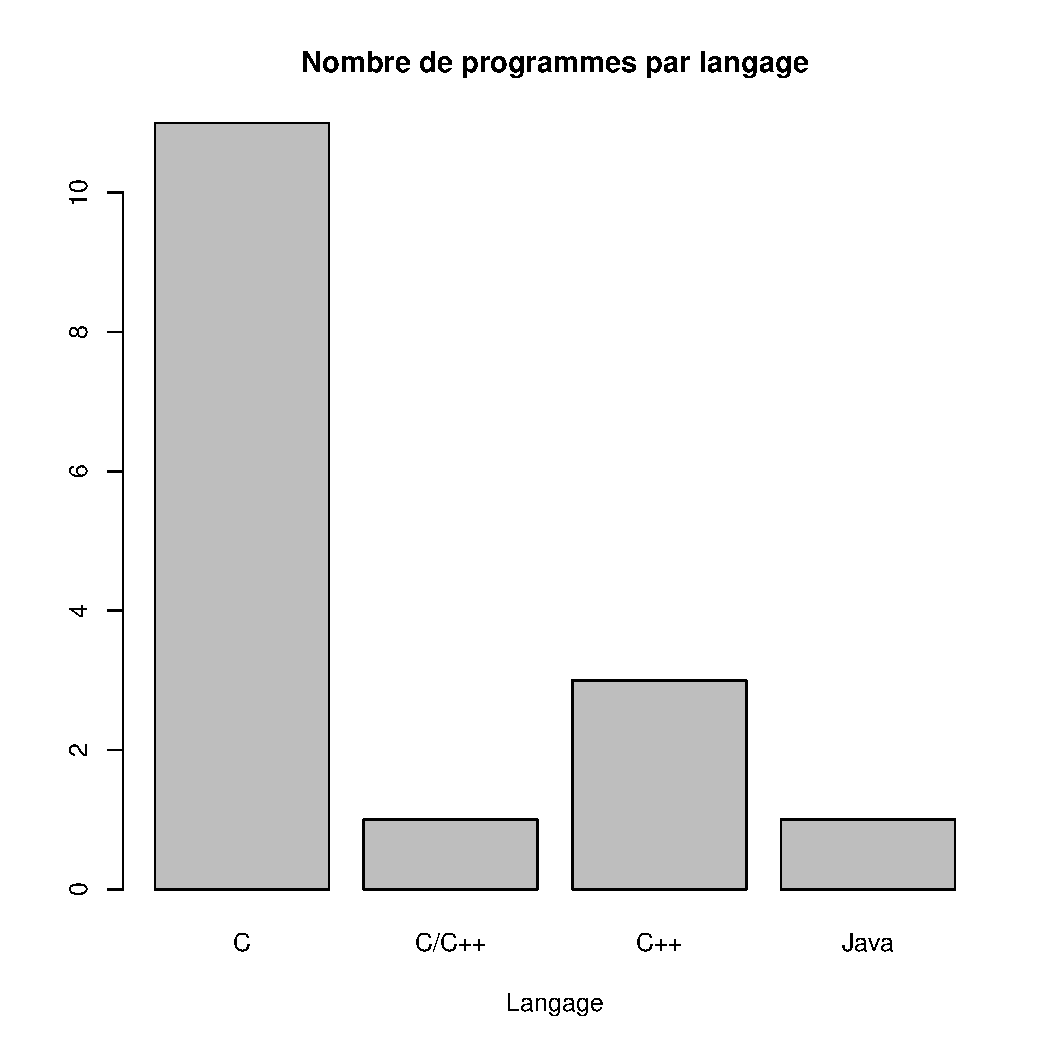
\includegraphics[width=\linewidth]{figures/prog_lang.pdf}
  \caption{}\label{fig:prog_lang}
  \endminipage\hfill
  \minipage{0.48\textwidth}
  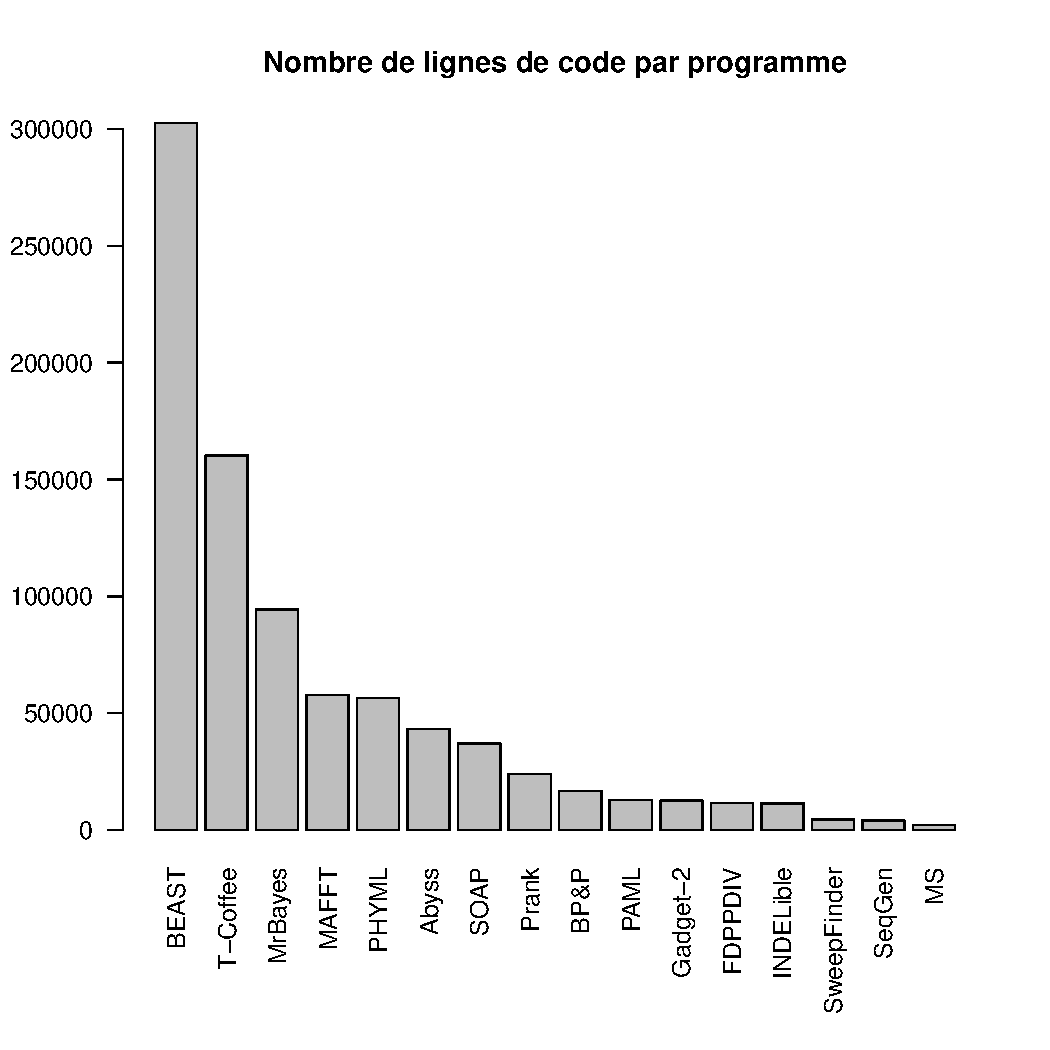
\includegraphics[width=\linewidth]{figures/lin_prog.pdf}
  \caption{}\label{fig:lin_prog}
  \endminipage\hfill
  \minipage{0.48\textwidth}
  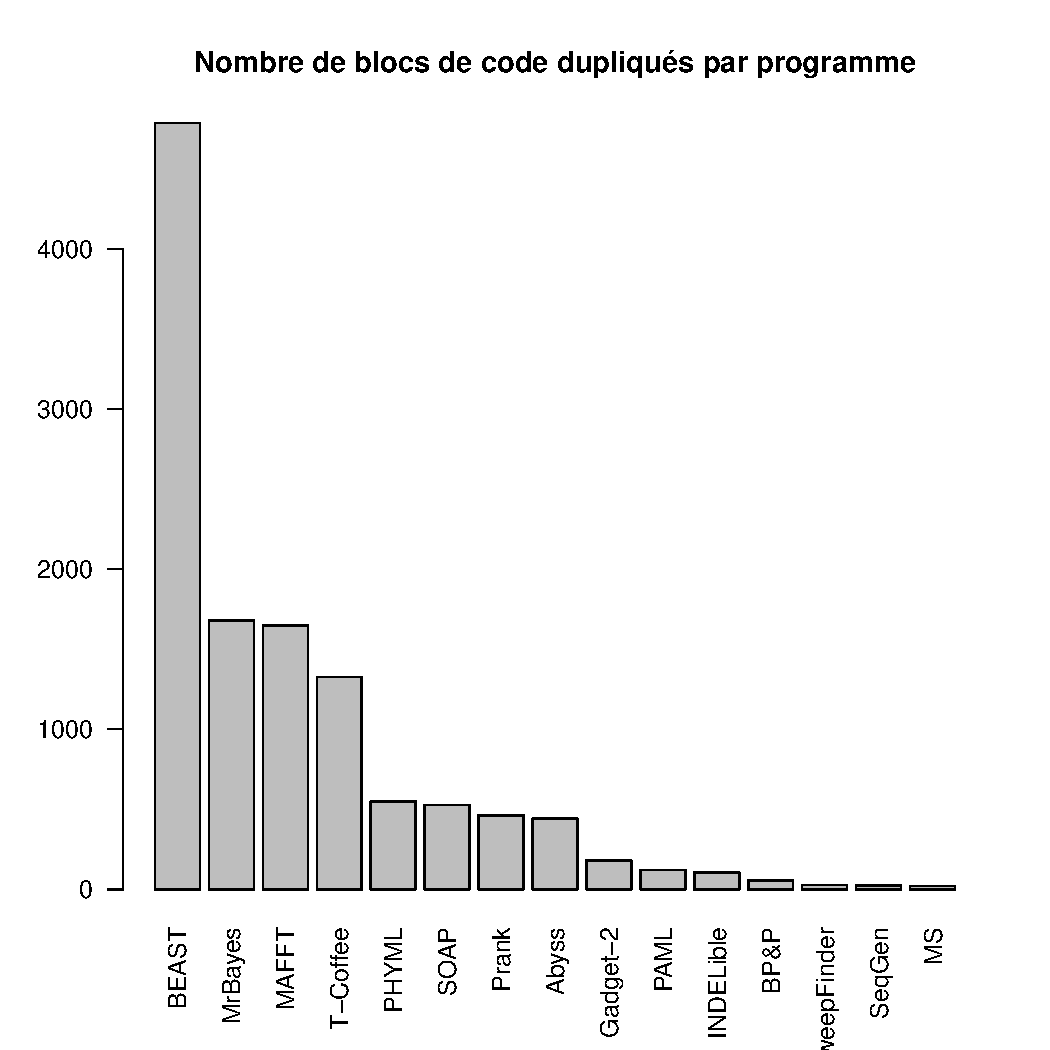
\includegraphics[width=\linewidth]{figures/dbl_prog.pdf}
  \caption{}\label{fig:dbl_prog}
  \endminipage\hfill
  \minipage{0.48\textwidth}
  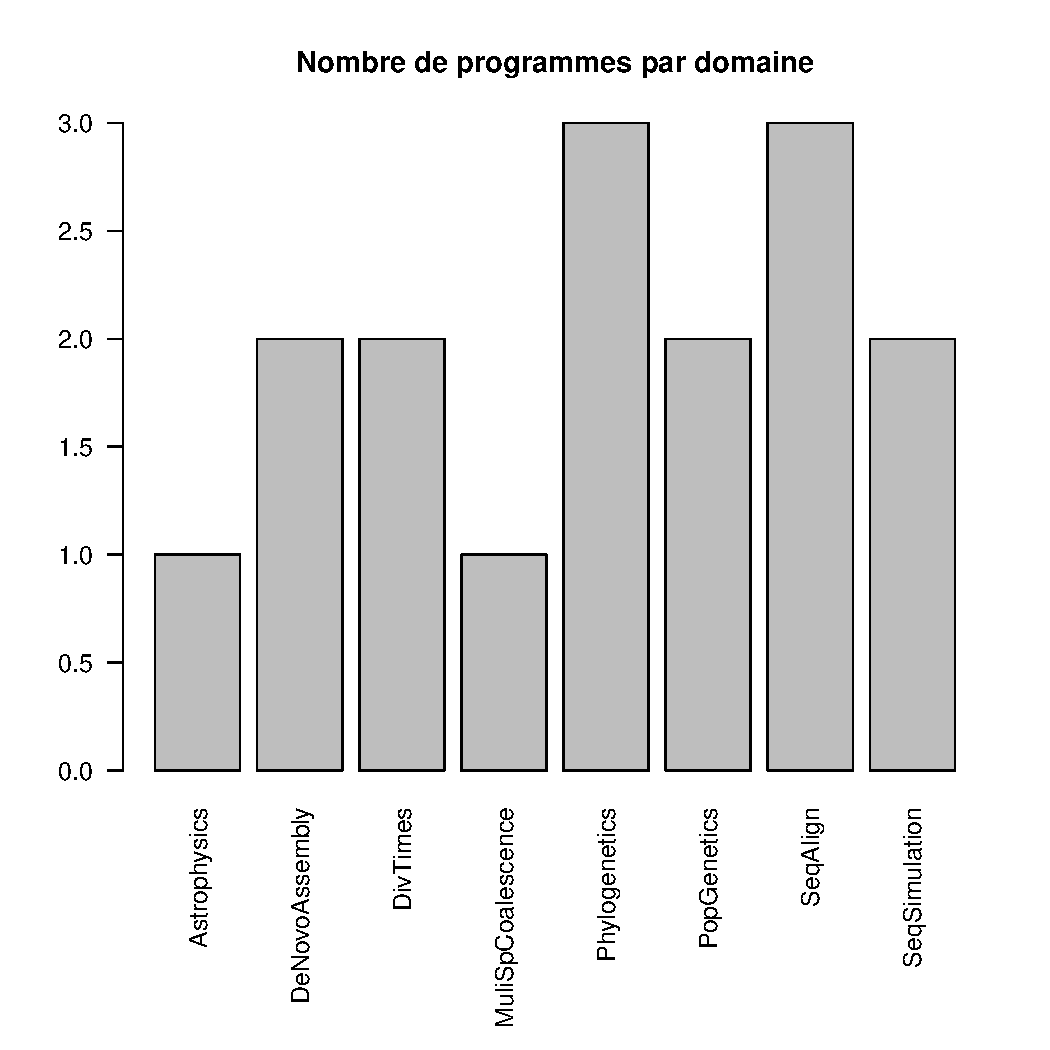
\includegraphics[width=\linewidth]{figures/prog_dom.pdf}
  \caption{}\label{fig:prog_dom}
  \endminipage\hfill
\end{figure}

\section{Pourcentage de lignes de code dupliquées}
Afin de calculer le pourcentage de ligne dupliquées, nous avons créé
une nouvelle table, contenant les noms des programmes, leurs
dommaines, les langages dans lesquels ils ont été écrits et leurs
nombres de lignes dupliquées (figure \ref{fig:dlin_prog}) ainsi que
leurs nombres de lignes totales. Nous avons enlevé de cette nouvelle
table de données les programmes pour ayant un champs non renseigné (à
l'aide de la commande \emph{na.omit}). Nous avons ensuite rajouté une
colonne à celle ci contenant les pourcentages de lignes de codes
dupliquées, avant de créer un histogrammes de ces pourcentages pour
chaque programme, ordonné par ordre décroissant (figure
\ref{fig:pdlin_prog}).

\begin{figure}[!h]
  \minipage{0.48\textwidth}
  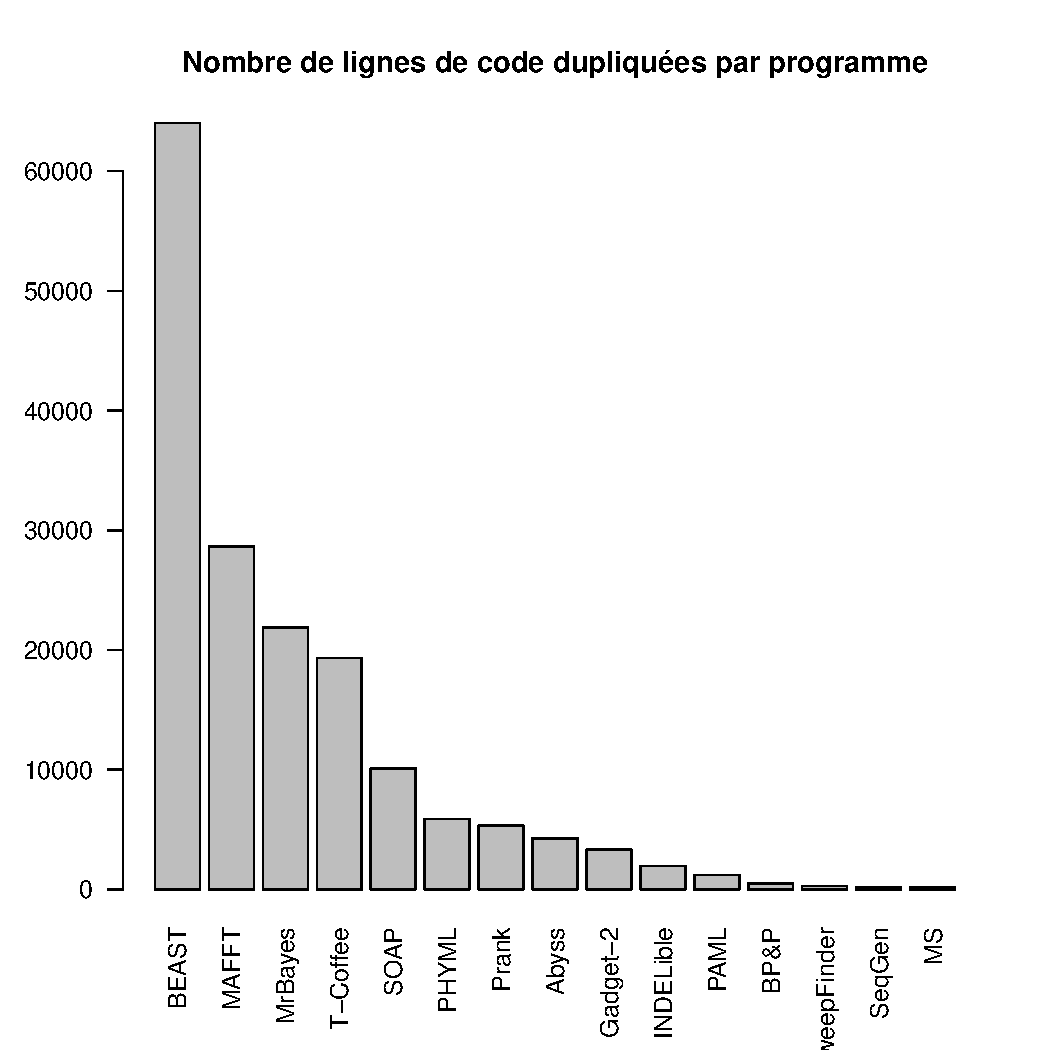
\includegraphics[width=\linewidth]{figures/dlin_prog.pdf}
  \caption{}\label{fig:dlin_prog}
  \endminipage\hfill
  \minipage{0.48\textwidth}
  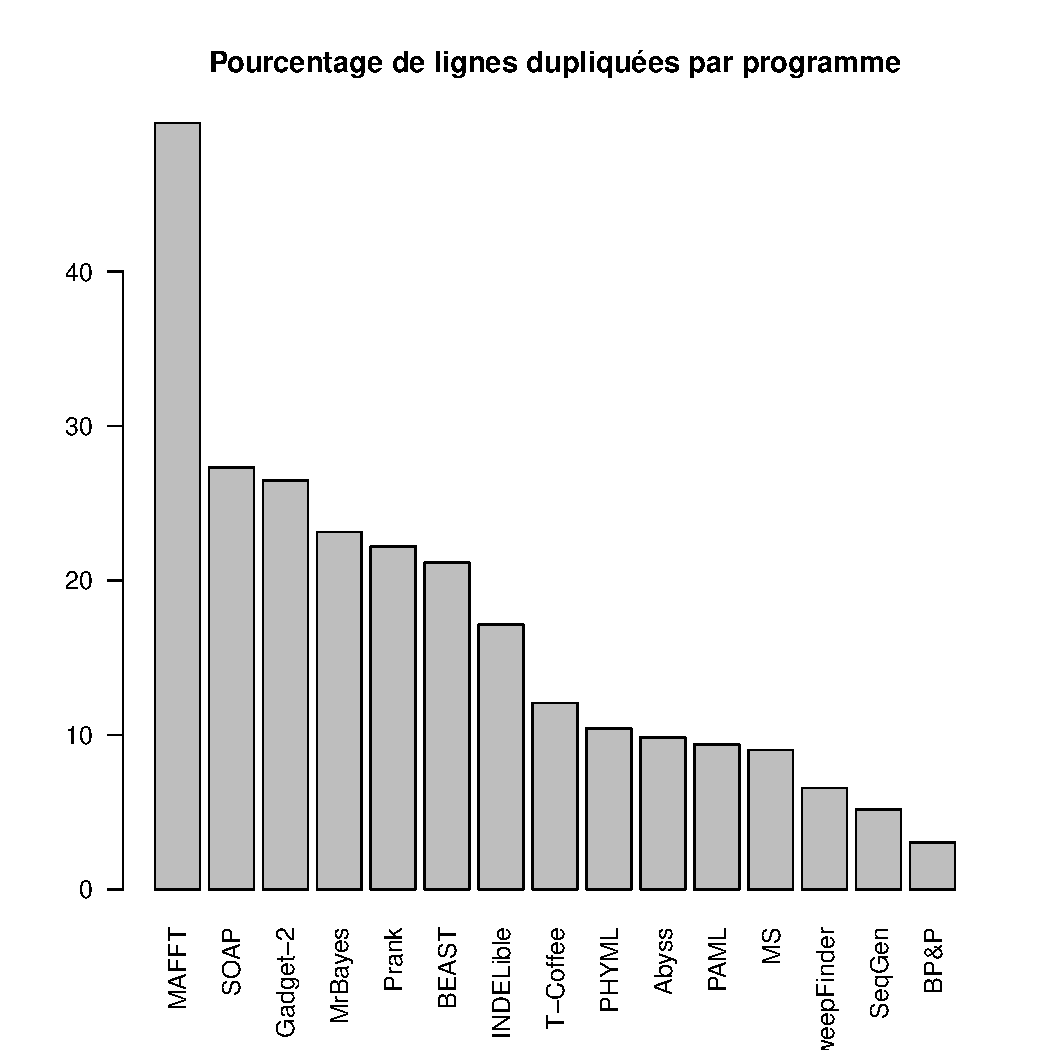
\includegraphics[width=\linewidth]{figures/pdlin_prog.pdf}
  \caption{}\label{fig:pdlin_prog}
  \endminipage\hfill
\end{figure}

\section{Comparaison du nombre de lignes duppliquées en C et en C++}
Pour effectuer un comparaison sur le nombre de lignes de code
dupliquées des programmes C et C++, il nous faut faire un test de
Mann-Whitney (grâce à la fonction \emph{wilcox.test} en R. Pour que ce
test soit valide, nous sommes obligés de supposer que les deux
échantillons considérés suivent une loi normale, de variance
identique. De plus, les mesures sont bien indépendantes les unes des
autres.

Nous faisons pour hypothèse nulle ``Il n'y a pas de différence
significative du nombre de lignes de code dupliquées en fonction du
langage de programmation utilisé.''. La p-value retournée par le test
est de 0.1608, au risque d'erreur 5\%, nous ne pouvons donc pas rejeter
l'hypothèse nulle. Nous en concluons que le nombre de lignes de code
dupliquées et le langage de programmation sont décorrélés.

Nous noterons que la longueur des codes biaise l'interprétation de la
mesure: en effet, plus un code est long, plus le nombre de lignes
dupliquées a de chance d'être élevé, aussi, un grand nombre de lignes
de code dupliquées ne reflète pas une mauvaise technique de
programmation, tout dépend de la taille du code!  Nous avons donc
aussi comparé le pourcentage des lignes de code dupliquées pour les
programmes écrits en C et en C++.

L'hypothèse nulle devient ``Il n'y a pas de différence significative
du pourcentage de lignes de code dupliquées en fonction du langage de
programmation utilisé.''.  La p-value retournée par le test est de
0.07692, au risque d'erreur 5\%, nous ne pouvons donc toujours pas
rejeter l'hypothèse nulle. Nous en concluons que le langage de
programmation et le pourcentage de lignes de code dupliquées sont
décorréllés.



\section{Intervalle de confiance du taux de lignes duppliquées}
L'intervalle de confiance à 90 \% du taux de lignes dupliquées est
obtenu grâce à la fonction \lstinline{t.test}. Il vaut [12.22694; 27.40435]
pour les programmes écrits en C++ et [1.264158; 21.246497] pour les
autres. La fonction \lstinline{t.test} renvoie aussi les moyennes des
échantillons.


\section{Lien entre la longueur du code et le nombre de warning à la
  compilation}
Nous voulons explorer l'hypothèse selon laquelle les codes longs
comporteraient plus de warnings à la compilation que les courts. Nous
avons commencé par séparer notre table en deux, l'une pour les
programmes au nombre de lignes de code inférieur à la médiane et
l'autre pour les autres programmes. 

Nous avons ensuite effectué trois tests de Mann Whitney, un pour chaque
type de warning (Clang, MinorWarning de gcc, MajorWarning de gcc),
avec pour hypothèse nulle ``Il n'y a pas de différence significative
du nombre de warnings à la compilation entre les programmes de
longueurs supérieures et inférieures à la médiane.''. Nous avons pour
cela encore une fois supposé que les échantillons considérés suivaient
une loi normale de variance identique. Lors du test, nous avons passé
\emph{alternative = "less"} en argument à la fonction
\emph{wilcox.test}, cela correspond au fait que nous nous attendons à
ce que le nombre de warnings soit supérieur pour pour les programmes
long.

Pour les Warning Clang, la p-value retournée par le test est de
0.0006216, au risque d'erreur 5\%, nous pouvons donc rejeter
l'hypothèse nulle. Nous en concluons que le nombre de warnings Clang
est supérieur pour les programmes longs.

Pour les Warning gcc, la p-value retournée par le test est de 0.7749
et 0.08464 pour les warning mineurs et majeurs respéctivement. Au
risque d'erreur 5\%, nous ne pouvons donc pas rejeter l'hypothèse
nulle. Nous en concluons que le nombre de warnings gcc n'est pas
significativement supérieur pour les programmes longs.

Le test de Mann Whitney étant un test de comparaison de moyennes, nous
avons voulu approfondir le lien entre le nombre de warnings Clang et la
taille des programmes. Pour cela, nous avons décider de faire un test de
corrélation entre ces deux grandeurs. Nous avons pour cela effectué un
test paramétrique de corrélation de Pearson avec la fonction
\emph{cor.test}. Ce test nécéssite que les données suivent une loi
normale, cette condition étant ici discutable, nous avons aussi
effectué un test non-paramétrique : le test de
corrélation de Spearman, disponible avec la même fonction. 

Le test de Pearson renvoie une p-value de 0.03095, et le test de
Spearman de 0.001907. Nous pouvons donc affirmer au risque d'erreur 5 \%
que le nombre de lignes de codes et le nombre de warnings Clang sont
corrélés.

Nous avons donc généré un graphique représentant le nombre de warnings
Clang en fonction du nombre de lignes de code, sur lequel nous avons
tracé une régression linéaire (figure \ref{fig:clang_lin}).


\begin{figure}[h]
  \centering
  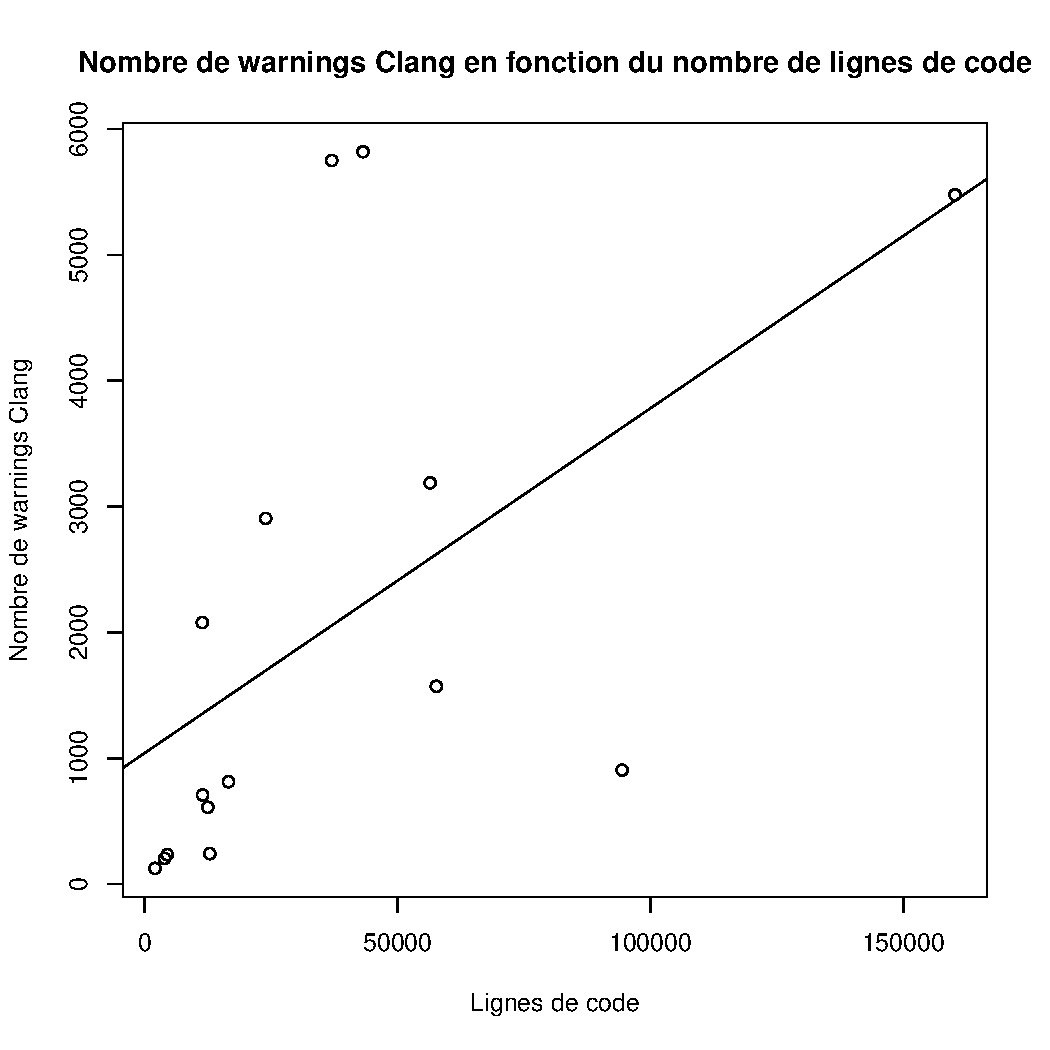
\includegraphics[width=.48\textwidth]{figures/clang_lin.pdf}
  \caption{}\label{fig:clang_lin}
\end{figure}

\section{Questions personnelles}
\subsection{Lien entre le nombre et le type de warning à la
  compilation et la qualité de la gestion mémoire.}
Nous avons choisi de nous demander si il existe un lien entre le
nombre de warnings de chaque type renvoyés pendant la compilation et la
qualité de la gestion mémoire attribuée par valgrind.

Nous pour cela séparé notre jeu de données en deux: les programmes
ayant une gestion mémoire décrite comme clean par valgrind, et les
autres.
Nous avons ensuite effectué trois tests de Mann Whitney, un pour chaque
type de warning (Clang, MinorWarning de gcc, MajorWarning de gcc),
avec pour hypothèse nulle ``Il n'y a pas de différence significative
du nombre de warnings à la compilation entre les programmes en fonction
de la qualité de leur gestion mémoire.''.

Pour les Major Warning, la p-value retournée par le test est de
0.02165, au risque d'erreur 5\%, nous pouvons donc rejeter
l'hypothèse nulle. Nous en concluons que le nombre de warnings majeur gcc
est supérieur pour les programmes ayant une gestion mémoire non propre
(figure \ref{fig:MW_valgr}).

\begin{figure}[h]
  \centering
  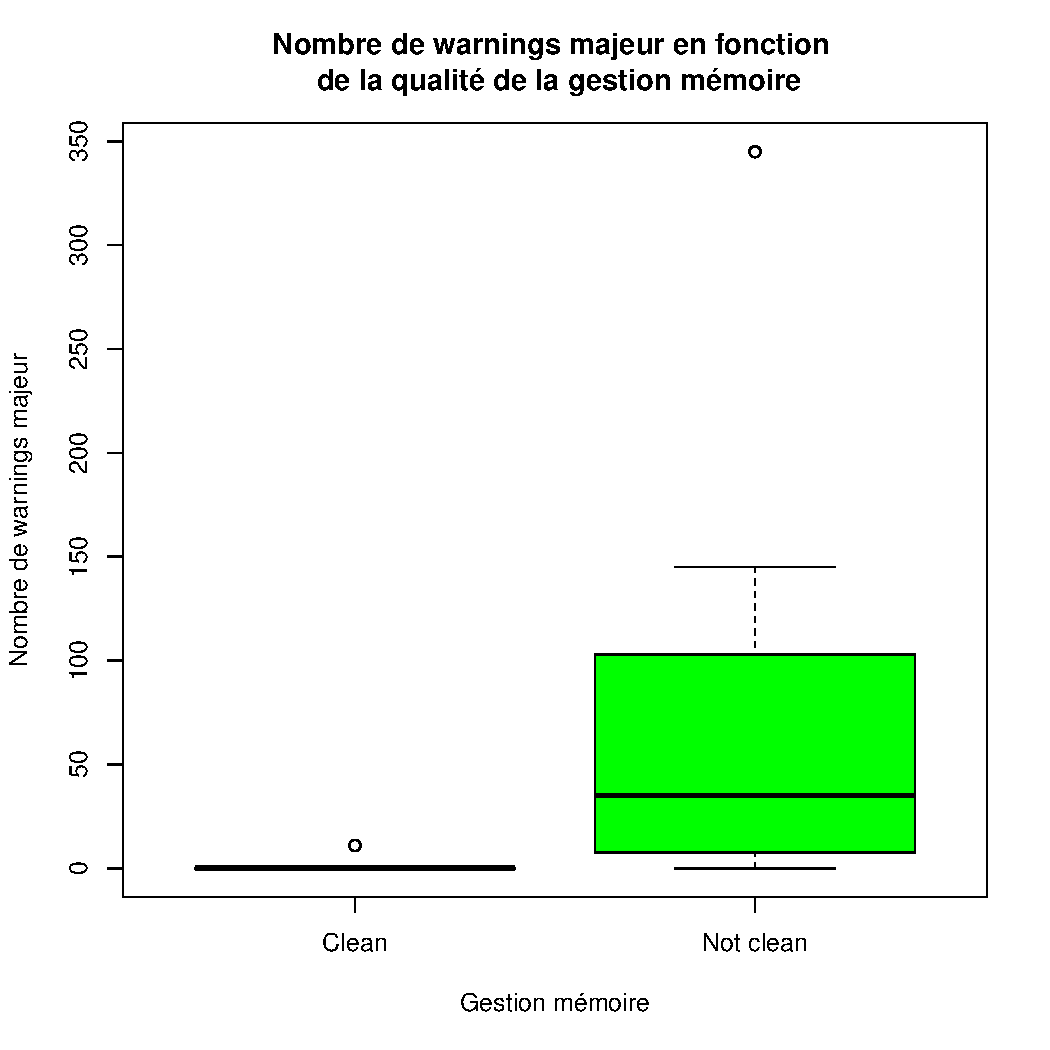
\includegraphics[width=.48\textwidth]{figures/MW_valgr.pdf}
  \caption{}\label{fig:MW_valgr}
\end{figure}

Pour les Warning mineurs et Clang respectivement, la p-value retournée
par le test est de 0.1645 et 0.7348. Au risque d'erreur 5\%, nous ne
pouvons donc pas rejeter l'hypothèse nulle. Nous en concluons que le
nombre de warning mineur gcc et clang n'est pas sensiblement inférieur
pour les programmes propres.

\subsection{Autre question}
Enfin, nous avons cherché à déterminer si les programmes d'un domaine en
particulier comportait une proportion plus importante de lignes
dupliquées. Nous avons pour cela effectué un test de Kruskal-Wallis
sur le pourcentage de lignes dupliquées par programme en fonction du
domaine.

L'hypothèse nulle est ``Il n'y a pas de différence significative du
pourcentage de lignes de code dupliquées en fonction du domaine
considéré.'' La p-value retournée par le test est de 0.2814, nous ne
pouvons donc pas rejeter l'hypothèse nulle au risque de 5 \%. Nous en
concluons que le domaine et le pourcentage de lignes de code
dupliquées ne sont pas liés. 


\section*{Annexe}
\lstinputlisting{../fusion.R}

\end{document}
